\documentclass[10pt]{beamer}

% Theme
\usetheme{default}
\usecolortheme{default}

% Add slide numbers in bottom left corner
\setbeamertemplate{footline}{
  \vspace*{0.5em}\hspace*{0.5em}\insertframenumber\hfill\vspace*{0.5em}
}

% Packages
\usepackage{graphicx}
\usepackage{amsmath}
\usepackage{amssymb}
\usepackage{booktabs}
\usepackage{xcolor}

% Title information
\title{Reproducing ``Bilinear MLPs Enable Weight-Based Mechanistic Interpretability''}
\author{Itay Erlich, May Ben Zion, Jacob Shashoua, Sagi Schwartz}
\date{FACT-AI Course Project \\ \today}

% Math commands (simplified from report)
% Save original checkmark and redefine with color
\let\oldcheckmark\checkmark
\renewcommand{\checkmark}{\textcolor{green!70!black}{\oldcheckmark}}
\newcommand{\vx}{\mathbf{x}}
\newcommand{\vy}{\mathbf{y}}
\newcommand{\vv}{\mathbf{v}}
\newcommand{\vW}{\mathbf{W}}
\newcommand{\vB}{\mathbf{B}}
\newcommand{\vl}{\boldsymbol{\lambda}}
\newcommand{\R}{\mathbb{R}}

\begin{document}

% Title slide
\begin{frame}
    \titlepage
\end{frame}

% Include slide files
% Introduction Slides

\begin{frame}{Bilinear MLPs: Weight-Based Interpretability}
    \begin{columns}
        \column{0.5\textwidth}
        \textbf{Purpose:}
        \begin{itemize}
            \item Direct interpretability from weights
            \item No post-hoc analysis needed
            \item No SAE training required
        \end{itemize}
        
        \vspace{0.3cm}
        \textbf{Key Insight:}\\
        Bilinear structure creates \textbf{quadratic} interactions that can be \textbf{eigendecomposed} to reveal interpretable input directions.
        
        \column{0.5\textwidth}
        \textbf{Method:}
        \begin{itemize}
            \item Replace nonlinearity with element-wise multiplication
            \item This creates an \textbf{interaction matrix} for each output
            \item Eigendecompose to find dominant input directions
            \item Top eigenvectors = most important patterns
        \end{itemize}
    \end{columns}
\end{frame}

\begin{frame}{Mathematical Foundation}
    \small
    \textbf{Bilinear Layer:} $\mathbf{y} = (\mathbf{W}_l \mathbf{x}) \odot (\mathbf{W}_r \mathbf{x})$
    
    \vspace{0.15cm}
    \textbf{Output as Quadratic Form:} For each output $c$: \quad $y_c = \mathbf{x}^\top B_c \, \mathbf{x}$
    
    \vspace{0.05cm}
    where $B_c$ is the \textbf{interaction matrix}---captures how input pairs $(x_i, x_j)$ contribute to $y_c$.
    
    \vspace{0.15cm}
    \textbf{Eigendecomposition:} Symmetrize and decompose $B_c$:
    \begin{equation*}
        B_c = \sum_{r=1}^{d} \lambda_r^{(c)} \mathbf{v}_r^{(c)} (\mathbf{v}_r^{(c)})^\top
        \quad \Rightarrow \quad
        y_c = \sum_r \lambda_r (\mathbf{v}_r^\top \mathbf{x})^2
    \end{equation*}
    
    \vspace{-0.1cm}
    \footnotesize
    Eigenvectors $\mathbf{v}_r^{(c)} \in \mathbb{R}^{d_{\text{in}}}$ = interpretable input directions; eigenvalues $\lambda_r^{(c)}$ = importance.
    
    \vspace{0.15cm}
    \small
    \textbf{Effective Rank:} Measures spectral concentration (how many eigenvalues matter):
    \begin{equation*}
        \text{EffRank}(\boldsymbol{\lambda}) = \left( \frac{\|\boldsymbol{\lambda}\|_1}{\|\boldsymbol{\lambda}\|_2} \right)^2
    \end{equation*}
    
    \vspace{-0.15cm}
    \footnotesize
    Low effective rank $\Rightarrow$ few dominant eigenvectors $\Rightarrow$ more interpretable.
\end{frame}

\begin{frame}{Two Analysis Methods (Paper Section 3)}
    \textbf{The analysis method depends on what features are available:}
    
    \vspace{0.15cm}
    \begin{columns}
        \column{0.5\textwidth}
        \fcolorbox{blue!50}{blue!10}{
            \parbox{0.95\textwidth}{
                \small
                \textbf{Method A: No Prior Features}\\[0.1cm]
                (Vision, Section 4)
                
                \vspace{0.1cm}
                \textbf{Model:} Single bilinear MLP + linear head (MNIST/Fashion-MNIST).
                
                \vspace{0.1cm}
                Classes act as output features.\\
                Eigendecompose $B_c$ directly:
                \begin{equation*}
                    y_c = \sum_r \lambda_r (\mathbf{v}_r^\top \mathbf{x})^2
                \end{equation*}
                Eigenvectors $\mathbf{v}_r$ visualized as 28$\times$28 images.
            }
        }
        
        \column{0.5\textwidth}
        \fcolorbox{green!50}{green!10}{
            \parbox{0.95\textwidth}{
                \small
                \textbf{Method B: SAE Features}\\[0.1cm]
                (Language, Section 5)
                
                \vspace{0.1cm}
                \textbf{Model:} Transformer with bilinear MLPs (replacing standard MLPs) + pretrained SAEs.
                
                \vspace{0.1cm}
                SAEs $\to$ sparse features $\mathbf{z}^{\text{in}}, \mathbf{z}^{\text{out}}$.\\
                Build $Q_f$ per output feature $f$:
                \begin{equation*}
                    z^{\text{out}}_f \approx (\mathbf{z}^{\text{in}})^\top Q_f \, \mathbf{z}^{\text{in}}
                \end{equation*}
            }
        }
    \end{columns}
    
    \vspace{0.2cm}
    \centering
    \small
    \textbf{Both methods} use eigendecomposition to identify important input directions for each output.
\end{frame}

% Reproduction Slides

\begin{frame}{Vision Results: Claims V1--V3}
    \begin{columns}[T]
        % V1: Low-rank emergence
        \column{0.3\textwidth}
        \fcolorbox{blue!50}{blue!5}{
            \parbox{0.95\textwidth}{
                \centering
                \textbf{V1: Low-rank emergence} \checkmark
                
                \vspace{0.05cm}
                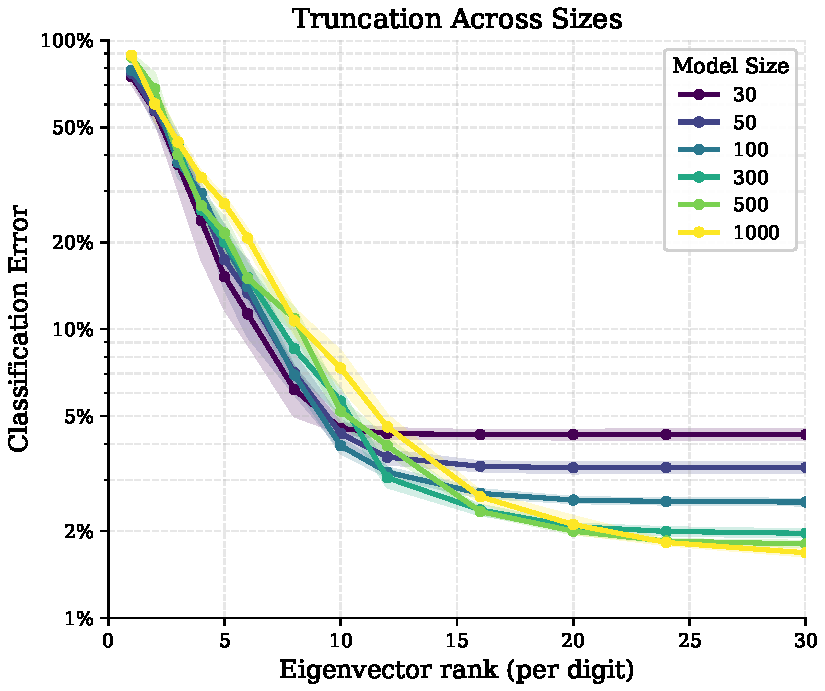
\includegraphics[width=0.95\textwidth,height=0.45\textheight,keepaspectratio]{../Report/figures/vision/figure_5b_truncation.pdf}
                
                \vspace{0.05cm}
                \scriptsize
                Top-$k$ truncation preserves accuracy
            }
        }
        
        % V2: Interpretable eigenvectors
        \column{0.35\textwidth}
        \fcolorbox{green!50}{green!5}{
            \parbox{0.95\textwidth}{
                \centering
                \textbf{V2: Interpretable eigenvectors} \checkmark
                
                \vspace{0.05cm}
                {\tiny Full Reg (noise+WD):}
                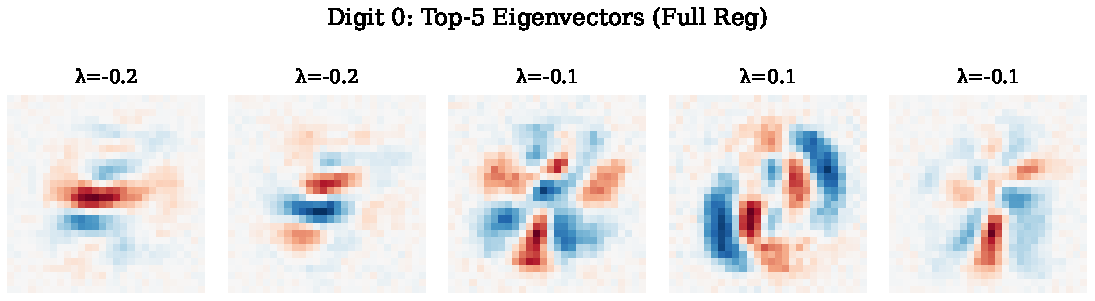
\includegraphics[width=0.95\textwidth,height=0.18\textheight,keepaspectratio]{../Report/figures/vision/eigenvectors_digit0_reg.pdf}
                
                \vspace{0.05cm}
                {\tiny Noise Only:}
                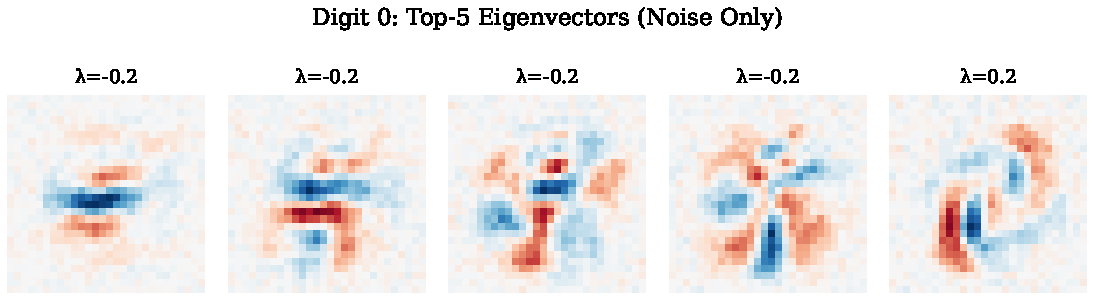
\includegraphics[width=0.95\textwidth,height=0.18\textheight,keepaspectratio]{../Report/figures/vision/eigenvectors_digit0_noise.pdf}
                
                \vspace{0.05cm}
                \scriptsize
                Both show clear ``0'' patterns
            }
        }
        
        % V3: Overfitting without reg
        \column{0.35\textwidth}
        \fcolorbox{red!50}{red!5}{
            \parbox{0.95\textwidth}{
                \centering
                \textbf{V3: Overfitting w/o reg} \checkmark
                
                \vspace{0.05cm}
                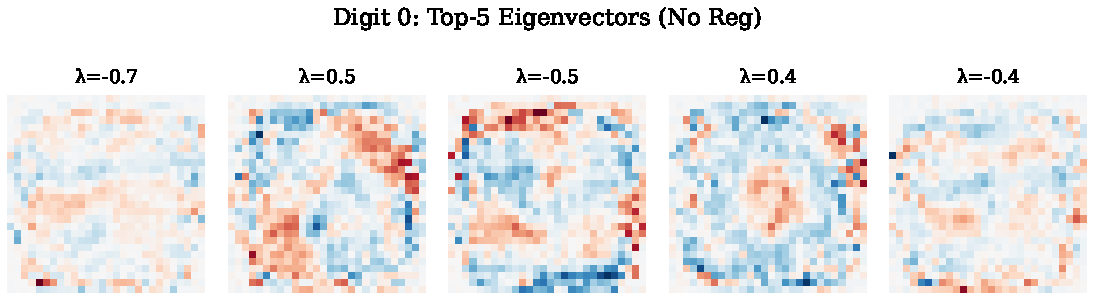
\includegraphics[width=0.95\textwidth,height=0.4\textheight,keepaspectratio]{../Report/figures/vision/eigenvectors_digit0_noreg.pdf}
                
                \vspace{0.05cm}
                \scriptsize
                Digit 0, no reg: diffuse, noisy
            }
        }
    \end{columns}
    
    \vspace{0.1cm}
    \centering
    \footnotesize
    \textbf{Key insight:} Regularization induces low-rank structure; \textbf{noise} makes eigenvectors interpretable.
\end{frame}

\begin{frame}{Vision Results: Claims V4--V6}
    \begin{columns}[T]
        % V4: Regularization roles
        \column{0.33\textwidth}
        \fcolorbox{blue!50}{blue!5}{
            \parbox{0.95\textwidth}{
                \centering
                \textbf{V4: Regularization roles} \checkmark
                
                \vspace{0.05cm}
                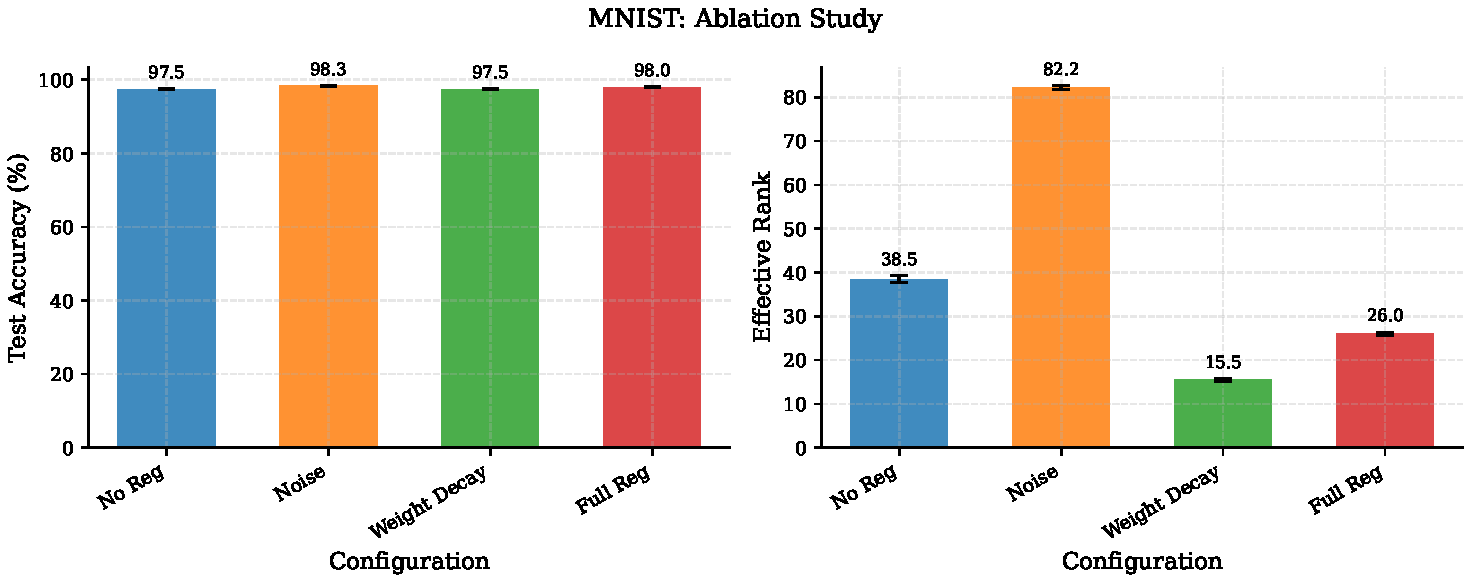
\includegraphics[width=0.95\textwidth,height=0.32\textheight,keepaspectratio]{../Report/figures/vision/mnist_ablation.pdf}
                
                \vspace{0.05cm}
                \scriptsize
                \textbf{WD} $\downarrow$ rank; \textbf{Noise} $\uparrow$ acc
                
                \vspace{0.05cm}
                \tiny
                EffRank ratio = $\frac{\text{EffRank(WD)}}{\text{EffRank(none)}}$\\
                $= \frac{15.5}{38.5} = 0.40 < 0.5$ \checkmark
            }
        }
        
        % V5: Cross-seed consistency
        \column{0.33\textwidth}
        \fcolorbox{green!50}{green!5}{
            \parbox{0.95\textwidth}{
                \centering
                \textbf{V5: Cross-seed consistency} \checkmark
                
                \vspace{0.05cm}
                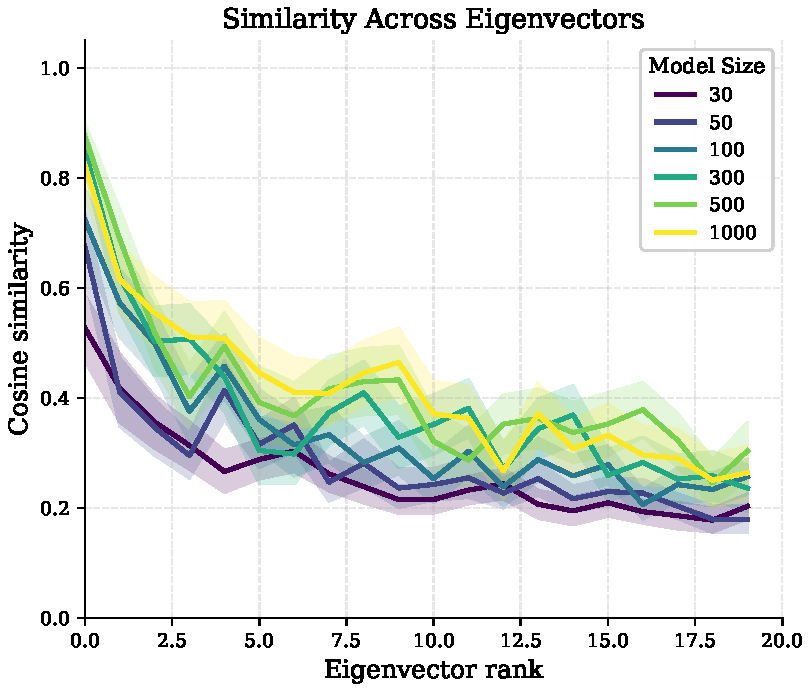
\includegraphics[width=0.95\textwidth,height=0.32\textheight,keepaspectratio]{../Report/figures/vision/figure_5a_similarity.pdf}
                
                \vspace{0.05cm}
                \scriptsize
                Top eigenvectors highly similar across seeds; similarity decays with rank
            }
        }
        
        % V6: Adversarial generation
        \column{0.33\textwidth}
        \fcolorbox{orange!50}{orange!5}{
            \parbox{0.95\textwidth}{
                \centering
                \textbf{V6: Adversarial gen.} \checkmark
                
                \vspace{0.05cm}
                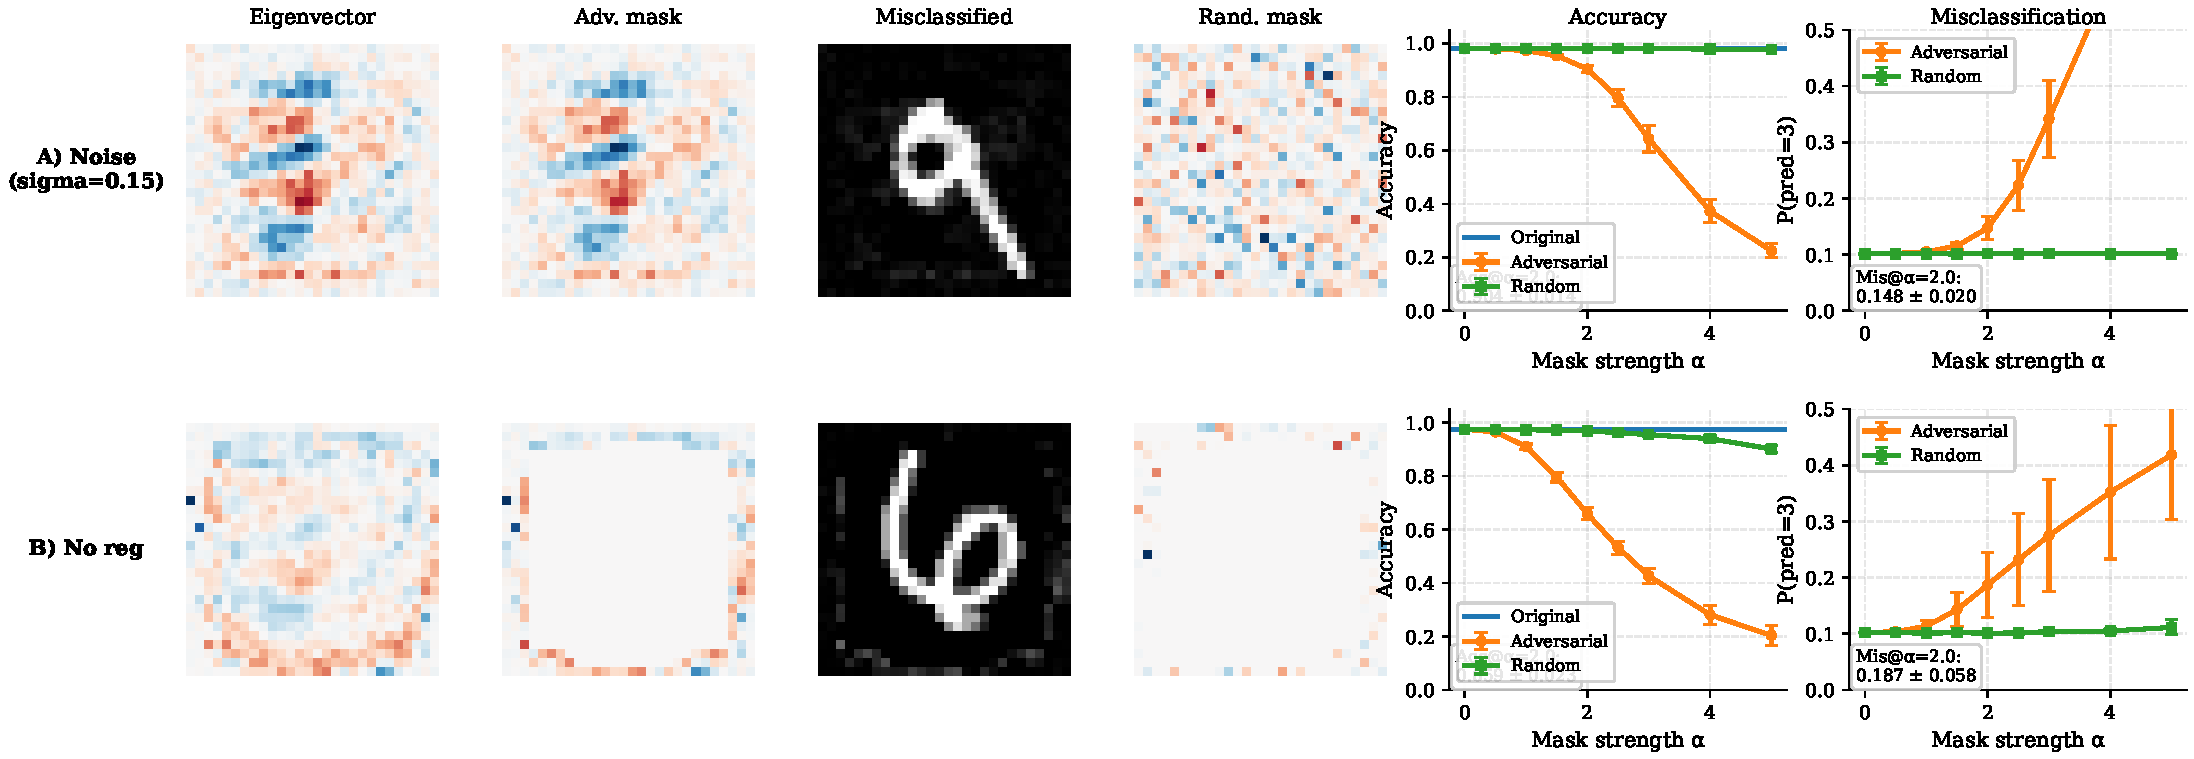
\includegraphics[width=0.95\textwidth,height=0.38\textheight,keepaspectratio]{../Report/figures/vision/figure_7_adversarial.pdf}
                
                \vspace{0.05cm}
                \scriptsize
                $\mathbf{m}_c = (V_c^+)^\dagger_{:,1}$: top positive eigenvector.\\
                Pseudoinverse extracts $V^+$ from $B_c$.\\
                \textbf{Result:} Eigenvector mask $>$ random.
            }
        }
    \end{columns}
    
    \vspace{0.1cm}
    \centering
    \footnotesize
    \textbf{All 6 vision claims reproduced.}
\end{frame}

\begin{frame}{Language Results: Claims L1, L2, L4 (Figure 8)}
    \begin{columns}[T]
        % LEFT: Methodology
        \column{0.32\textwidth}
        \small
        \textbf{Methodology:}
        
        \vspace{0.1cm}
        \scriptsize
        \textbf{1. Data:} Run $\sim$50k tokens, record MLP activations $\mathbf{h}^{\text{in}}, \mathbf{h}^{\text{out}}$.
        
        \vspace{0.05cm}
        \textbf{2. Encode:} Use pretrained SAEs:\\
        $\mathbf{z} = \text{TopK}(\mathbf{W}_{\text{enc}} \mathbf{h})$
        
        \vspace{0.05cm}
        \textbf{3. Build $Q_f$:} For output feature $f$:\\
        $z^{\text{out}}_f \approx (\mathbf{z}^{\text{in}})^\top Q_f \mathbf{z}^{\text{in}}$
        
        \vspace{0.05cm}
        \textbf{4. Analyze:} Eigendecompose $Q_f$, visualize structure.
        
        % RIGHT: Figure + Claims
        \column{0.68\textwidth}
        \centering
        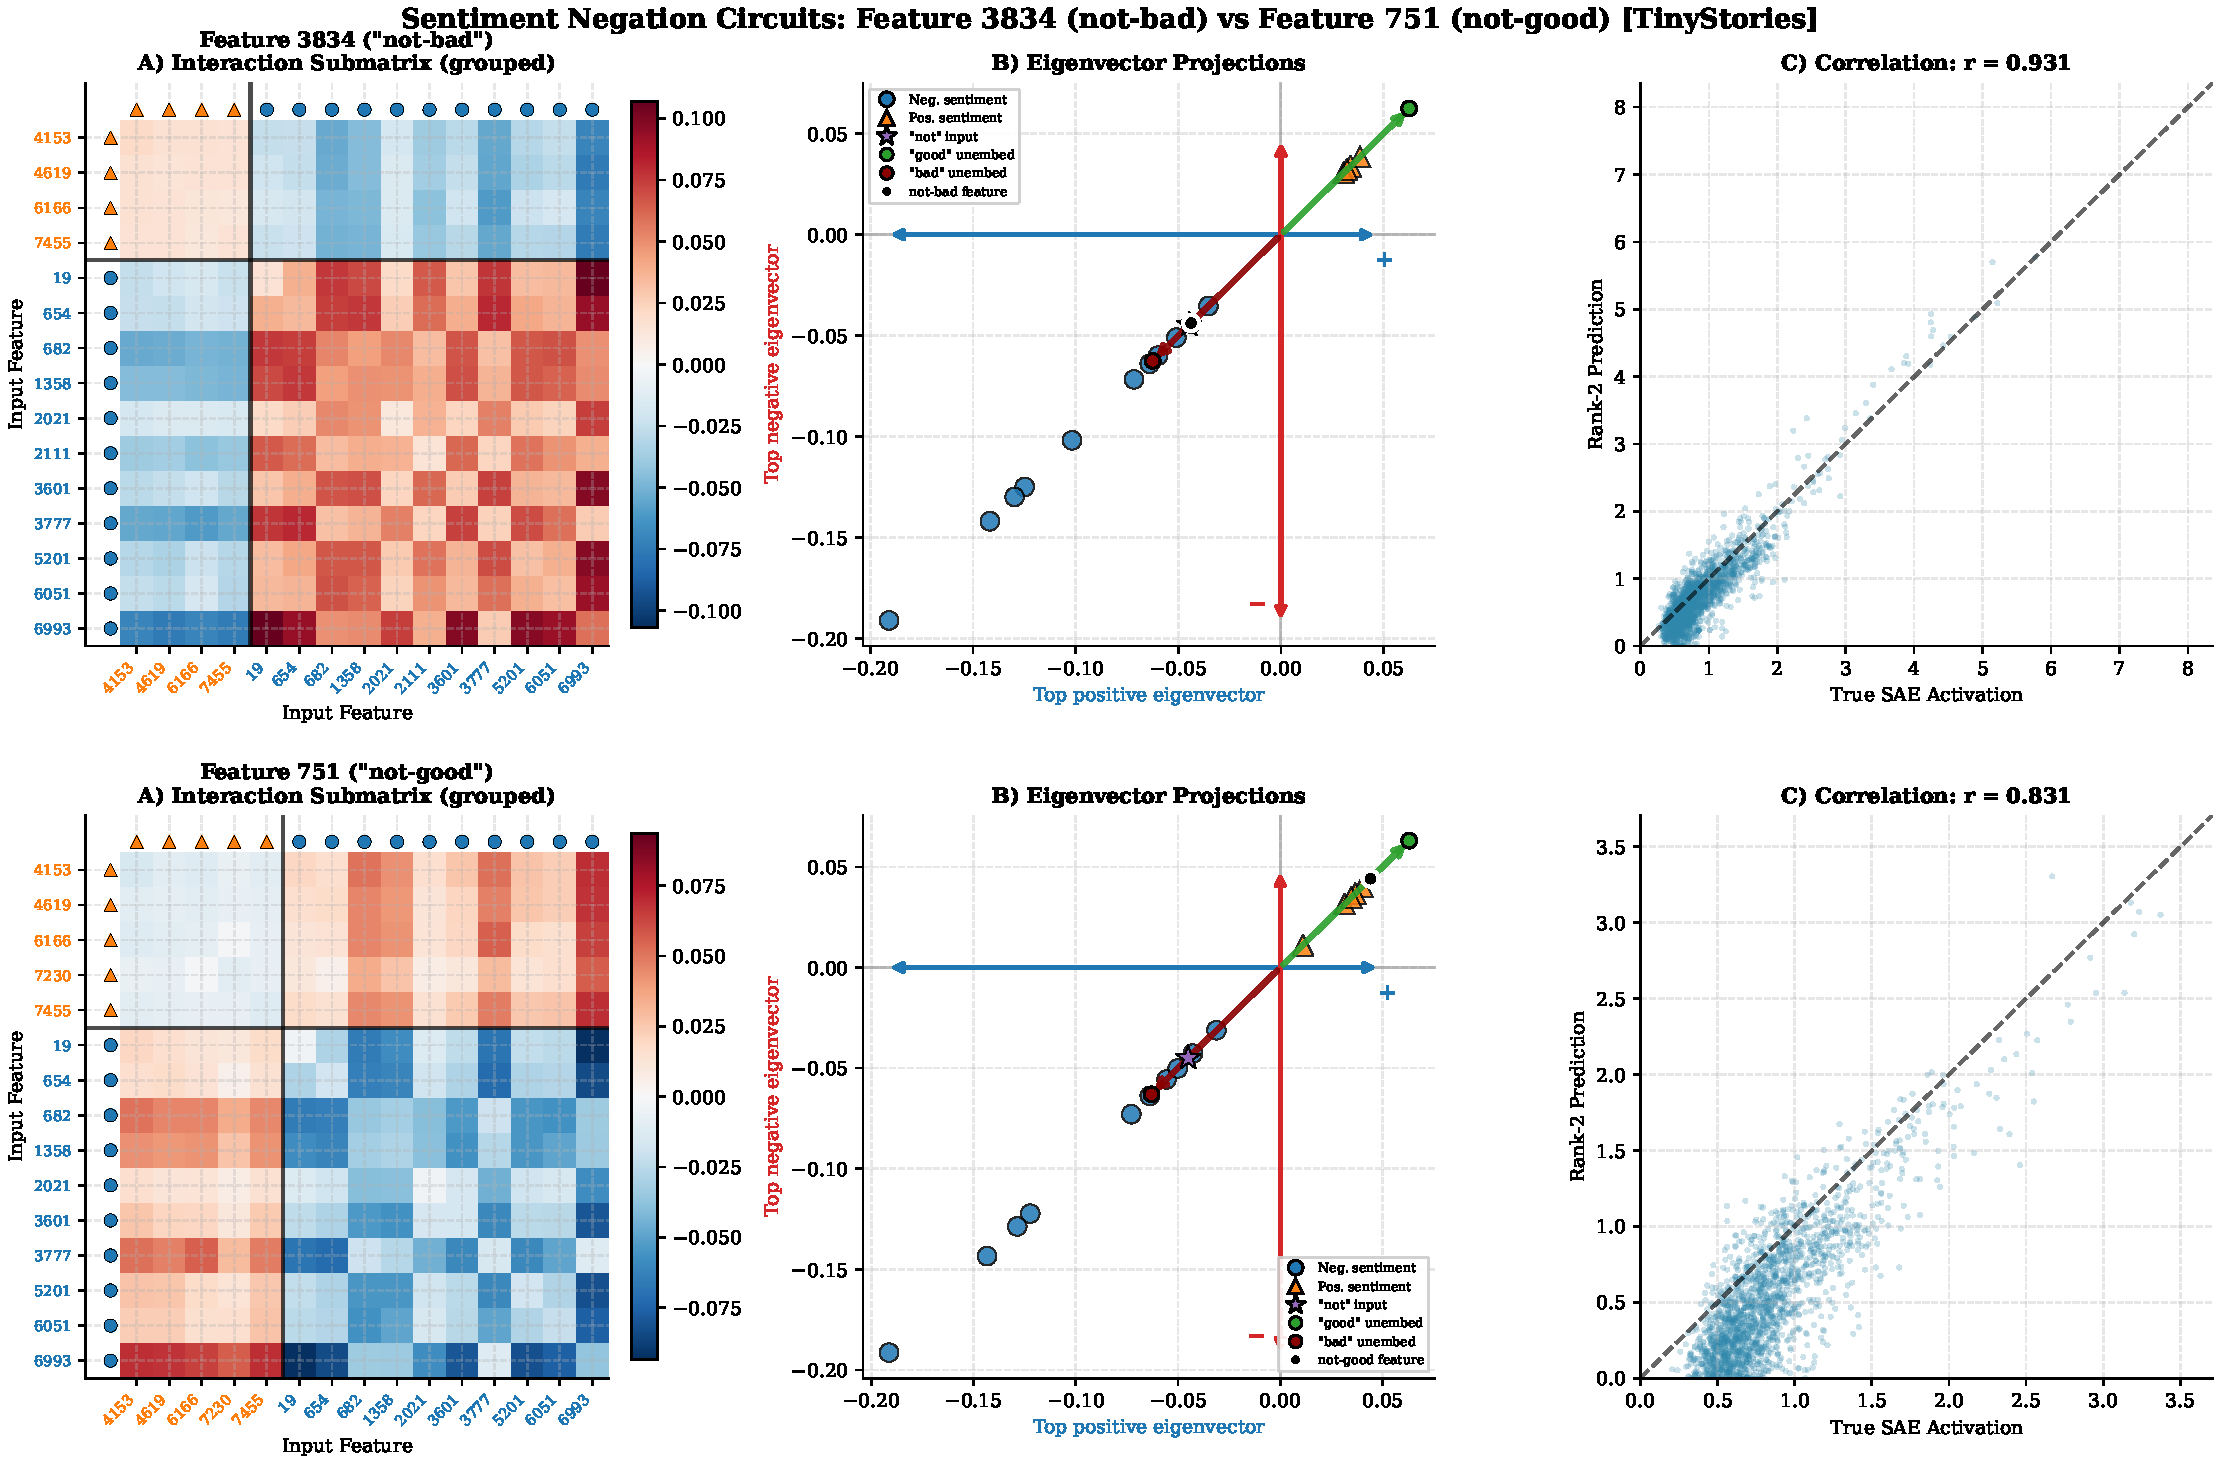
\includegraphics[width=\textwidth,height=0.38\textheight,keepaspectratio]{../Report/figures/language/figure_8_final.pdf}
        
    \end{columns}
    
    \vspace{0.1cm}
    \footnotesize
    \hspace{-0.3cm}
    \fcolorbox{blue!50}{blue!5}{
        \parbox{0.28\textwidth}{\scriptsize
            \textbf{L1: SAE discovery} \checkmark\\[0.05cm]
            SAEs find interpretable features (``not-good'', ``not-bad'')
        }
    }
    \hfill
    \fcolorbox{green!50}{green!5}{
        \parbox{0.28\textwidth}{\scriptsize
            \textbf{L2: Negation circuit} \checkmark\\[0.05cm]
            AND-gate confirmed: negation $\otimes$ sentiment
        }
    }
    \hfill
    \fcolorbox{orange!50}{orange!5}{
        \parbox{0.28\textwidth}{\scriptsize
            \textbf{L4: Sparse interact.} \checkmark\\[0.05cm]
            $Q_f$ shows clear block structure
        }
    }
    
    \vspace{0.1cm}
    \hrule
    \vspace{0.05cm}
    \scriptsize
    \textbf{Cosine similarity:} Paper reports $\cos = -0.975$ (ts-medium, L4). We get $\cos = -0.16$ (fw-medium, L7) --- weakly negative, not true opposites.\\
    \textbf{Model difference:} Paper uses ts-medium (L4, 4x SAE). We use fw-medium (L7, 8x SAE) because ts-medium lacks \texttt{mlp-in} SAEs on HuggingFace.
\end{frame}

\begin{frame}{Language Results: Claims L3, L5 (Figure 9)}
    % TOP: Explanation
    \small
    \textbf{What we measure (Figure 9):}
    \begin{columns}[T]
        \column{0.5\textwidth}
        \fcolorbox{blue!50}{blue!5}{
            \parbox{0.95\textwidth}{\scriptsize
                \textbf{L3: Low-rank emergence}\\[0.1cm]
                \textbf{Data:} $\sim$1.57M tokens $\to$ record $\mathbf{z}^{\text{in}}, \mathbf{z}^{\text{out}}$ per token.\\[0.05cm]
                \textbf{Filter:} Only \textbf{active} features ($z^{\text{out}}_f > 0$).\\[0.05cm]
                \textbf{Predict:} $\hat{z}^{\text{out}}_f = \sum_{r=1}^{k} \lambda_r (\mathbf{v}_r^\top \mathbf{z}^{\text{in}})^2$\\[0.05cm]
                \textbf{Measure:} Pearson corr $\Rightarrow$ high at $k$=2 = \textbf{low-rank}
            }
        }
        
        \column{0.5\textwidth}
        \fcolorbox{green!50}{green!5}{
            \parbox{0.95\textwidth}{\scriptsize
                \textbf{L5: Cross-model test}\\[0.1cm]
                \textbf{Paper:} ``most'' features corr $>$0.75\\[0.05cm]
                \textbf{Ours:}\\
                fw-small: 65\% (198 tok/param) \checkmark\\
                ts-medium: 32\% (83 tok/param)\\
                fw-medium: 45\% (99 tok/param)
            }
        }
    \end{columns}
    
    \vspace{0.1cm}
    % BOTTOM: Figures
    \begin{columns}[T]
        \column{0.4\textwidth}
        \centering
        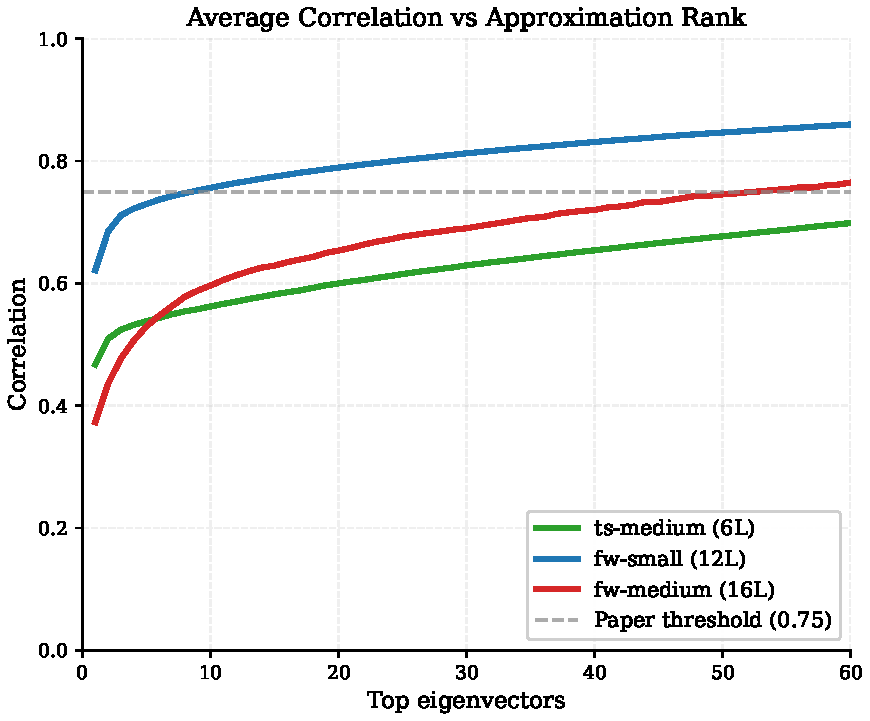
\includegraphics[width=\textwidth,height=0.32\textheight,keepaspectratio]{../Report/figures/language/figure_9a_correlation_progression.pdf}
        {\tiny Correlation vs rank $k$}
        
        \column{0.4\textwidth}
        \centering
        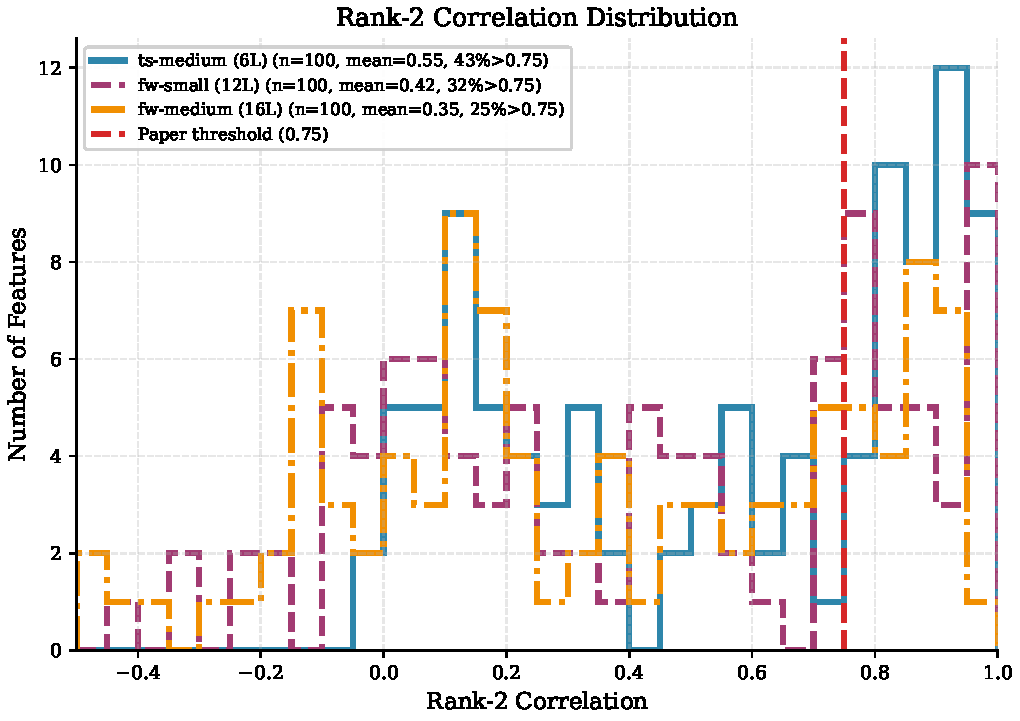
\includegraphics[width=\textwidth,height=0.32\textheight,keepaspectratio]{../Report/figures/language/figure_9b_correlation_histogram.pdf}
        {\tiny Rank-2 correlation histogram}
        
        \column{0.2\textwidth}
        \scriptsize
        \textbf{Why vary?}\\
        Higher tok/param $\to$ better low-rank behavior
        
        \vspace{0.1cm}
        \fcolorbox{black}{yellow!20}{
            \parbox{0.9\textwidth}{\tiny
                L3 $\sim$ \quad L5 $\sim$\\
                (partial)
            }
        }
    \end{columns}
\end{frame}

\begin{frame}{Language: Training Time Effect (Figure 10)}
    \begin{columns}[T]
        \column{0.55\textwidth}
        \centering
        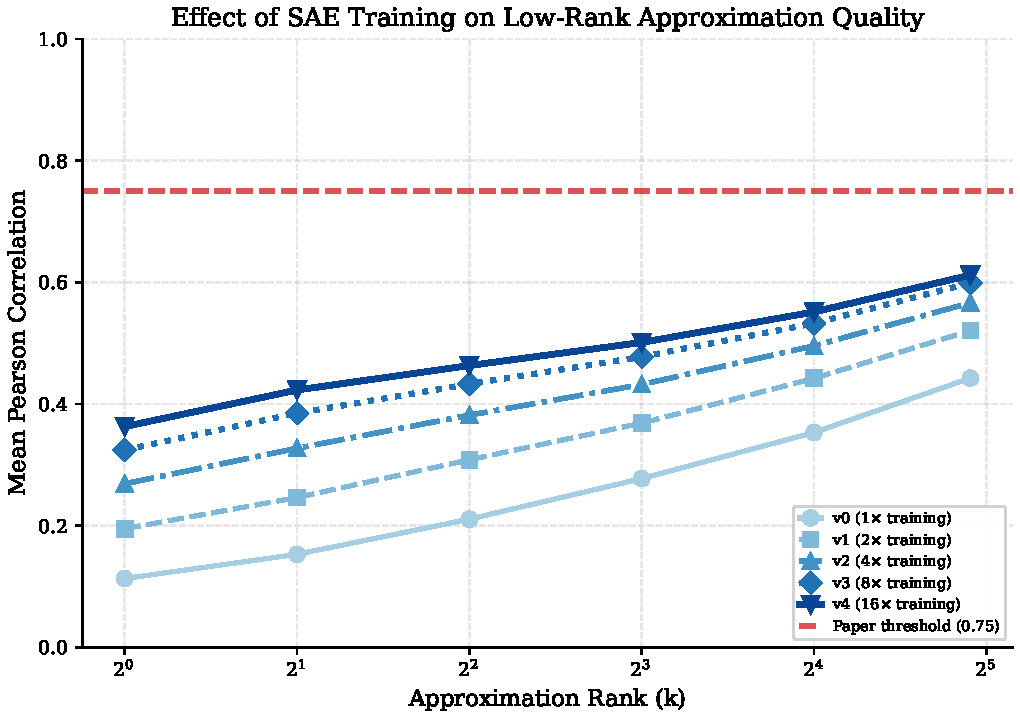
\includegraphics[width=\textwidth,height=0.55\textheight,keepaspectratio]{../Report/figures/language/figure_10a_sae_training_effect.pdf}
        
        \column{0.45\textwidth}
        \small
        \textbf{Hypothesis:} Low-rank emergence requires sufficient training.
        
        \vspace{0.2cm}
        \textbf{Evidence:} SAE training progression (v0 $\to$ v4) shows:
        \begin{itemize}
            \item Fraction of features with corr $>$ 0.75 increases \textbf{2.5$\times$}
            \item More training $\to$ better low-rank structure
        \end{itemize}
        
        \vspace{0.2cm}
        \textbf{Tokens/param ratio:}
        \begin{itemize}
            \item fw-small: 198 $\to$ 65\% high corr
            \item fw-medium: 99 $\to$ 45\%
            \item ts-medium: 83 $\to$ 32\%
        \end{itemize}
        
        \vspace{0.1cm}
        \scriptsize
        Models trained longer (higher tok/param) show stronger low-rank behavior.
    \end{columns}
\end{frame}

\begin{frame}{Reproduction Summary}
    \begin{table}[h]
        \centering
        \footnotesize
        \begin{tabular}{lp{3.5cm}cp{4cm}}
            \toprule
            ID & Description & Status & Notes \\
            \midrule
            \multicolumn{4}{c}{\textit{Vision (Section 4)}} \\
            \midrule
            V1 & Low-rank emergence & \checkmark & EffRank: 15.5 vs.\ 38.5 \\
            V2 & Interpretable eigenvectors & \checkmark & Clear digit patterns \\
            V3 & Overfitting without reg. & \checkmark & Diffuse patterns \\
            V4 & Regularization roles & \checkmark & WD $\downarrow$ rank; noise $\uparrow$ acc \\
            V5 & Cross-seed consistency & \checkmark & Top eigenvecs similar; acc low std \\
            V6 & Adversarial generation & \checkmark & Eigenvector attacks work \\
            \midrule
            \multicolumn{4}{c}{\textit{Language (Section 5)}} \\
            \midrule
            L1 & SAE feature discovery & \checkmark & Pretrained SAEs work \\
            L2 & Negation circuits & \checkmark & AND-gate confirmed \\
            L3 & Low-rank interactions & $\sim$ & 32--65\% $>$0.75 \\
            L4 & Sparse interactions & \checkmark & Block structure found \\
            L5 & Cross-model generalization & $\sim$ & Method works; varies \\
            \bottomrule
        \end{tabular}
    \end{table}
\end{frame}

% Extension 1: Cross-Dataset Robustness Slides

\begin{frame}{Extension 1: Background and Purpose}
    \textbf{Hypothesis:} Eigenvector decomposition generalizes across datasets
    
    \vspace{0.5cm}
    \textbf{Test Cases:}
    \begin{itemize}
        \item \textbf{Writer Independence:} MNIST $\leftrightarrow$ EMNIST-Digits
        \item \textbf{Domain Transfer:} MNIST $\rightarrow$ USPS (16$\times$16 $\to$ 28$\times$28)
        \item \textbf{Geometric Semantics:} MNIST $\rightarrow$ EMNIST-Letters
        \begin{itemize}
            \item O $\to$ 0, I $\to$ 1, Z $\to$ 2, S $\to$ 5
        \end{itemize}
    \end{itemize}
    
    \vspace{0.5cm}
    \textbf{Intuition:} Geometric resemblance should lead to similar eigenvectors
    
    \vspace{0.3cm}
    \small
    All models use Center-of-Mass (CoM) normalization to focus on shape geometry
\end{frame}

\begin{frame}{Extension 1: Results - Generalization Works!}
    \begin{columns}
        \column{0.5\textwidth}
        \textbf{Cross-Dataset Accuracy:}
        \begin{itemize}
            \item MNIST $\to$ EMNIST-Digits: \textbf{97.7\%}
            \item EMNIST-Digits $\to$ MNIST: \textbf{97.9\%}
        \end{itemize}
        
        \vspace{0.3cm}
        \textbf{USPS Transfer:}
        \begin{itemize}
            \item Regularized: \textbf{72.3\%}
            \item Baseline: 53.4\%
            \item Improvement: \textbf{+19 pp}
        \end{itemize}
        
        \column{0.5\textwidth}
        \textbf{Letter $\to$ Digit Mapping:}
        \begin{itemize}
            \item O $\to$ 0: \textbf{99.6\%}
            \item I $\to$ 1: \textbf{87.1\%}
            \item Z $\to$ 2: \textbf{88.8\%}
            \item S $\to$ 5: \textbf{87.4\%}
        \end{itemize}
    \end{columns}
\end{frame}

\begin{frame}{Extension 1: Eigenvector Comparison}
    \begin{center}
        \begin{figure}
            \centering
            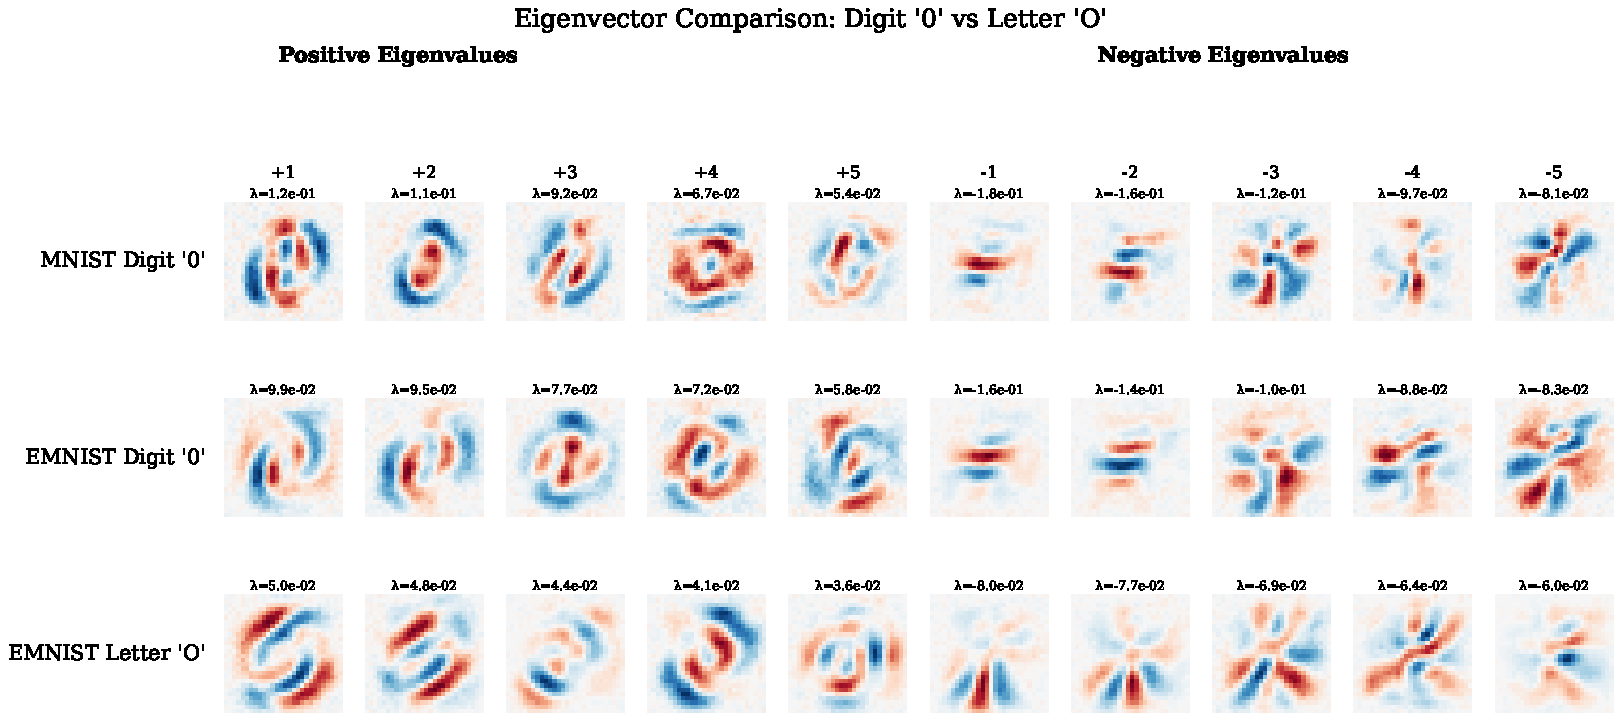
\includegraphics[width=0.9\textwidth]{../Report/figures/extension2/extension2_3way_comparison.pdf}
            \caption{Eigenvector Comparison: Digit '0' vs Letter 'O'}
        \end{figure}
    \end{center}
\end{frame}

\begin{frame}{Quadratic Form Similarity}
    \textbf{Problem:} Cosine similarity fails
    \begin{itemize}
        \item Similar pairs (0--O): 0.358
        \item Dissimilar pairs (0--X): 0.339
        \item Not discriminative!
    \end{itemize}
    
    \vspace{0.5cm}
    \textbf{Solution:} Quadratic Form Similarity
    \begin{equation*}
        \text{sim}(A, B) = \frac{\text{tr}(A \cdot B)}{\|A\|_F \|B\|_F} \in [-1, 1]
    \end{equation*}
    
    \vspace{0.3cm}
    \textbf{Results:}
    \begin{itemize}
        \item Similar pairs: \textbf{0.400}
        \item Dissimilar pairs: \textbf{-0.060}
        \item Large gap with $p < 10^{-4}$
    \end{itemize}
    
    \vspace{0.2cm}
    \small
    Incorporates eigenvalue signs and eigenvector alignment
\end{frame}

\begin{frame}{Extension 1: Quadratic Form Similarity Heatmap}
    \begin{center}
        \begin{figure}
            \centering
            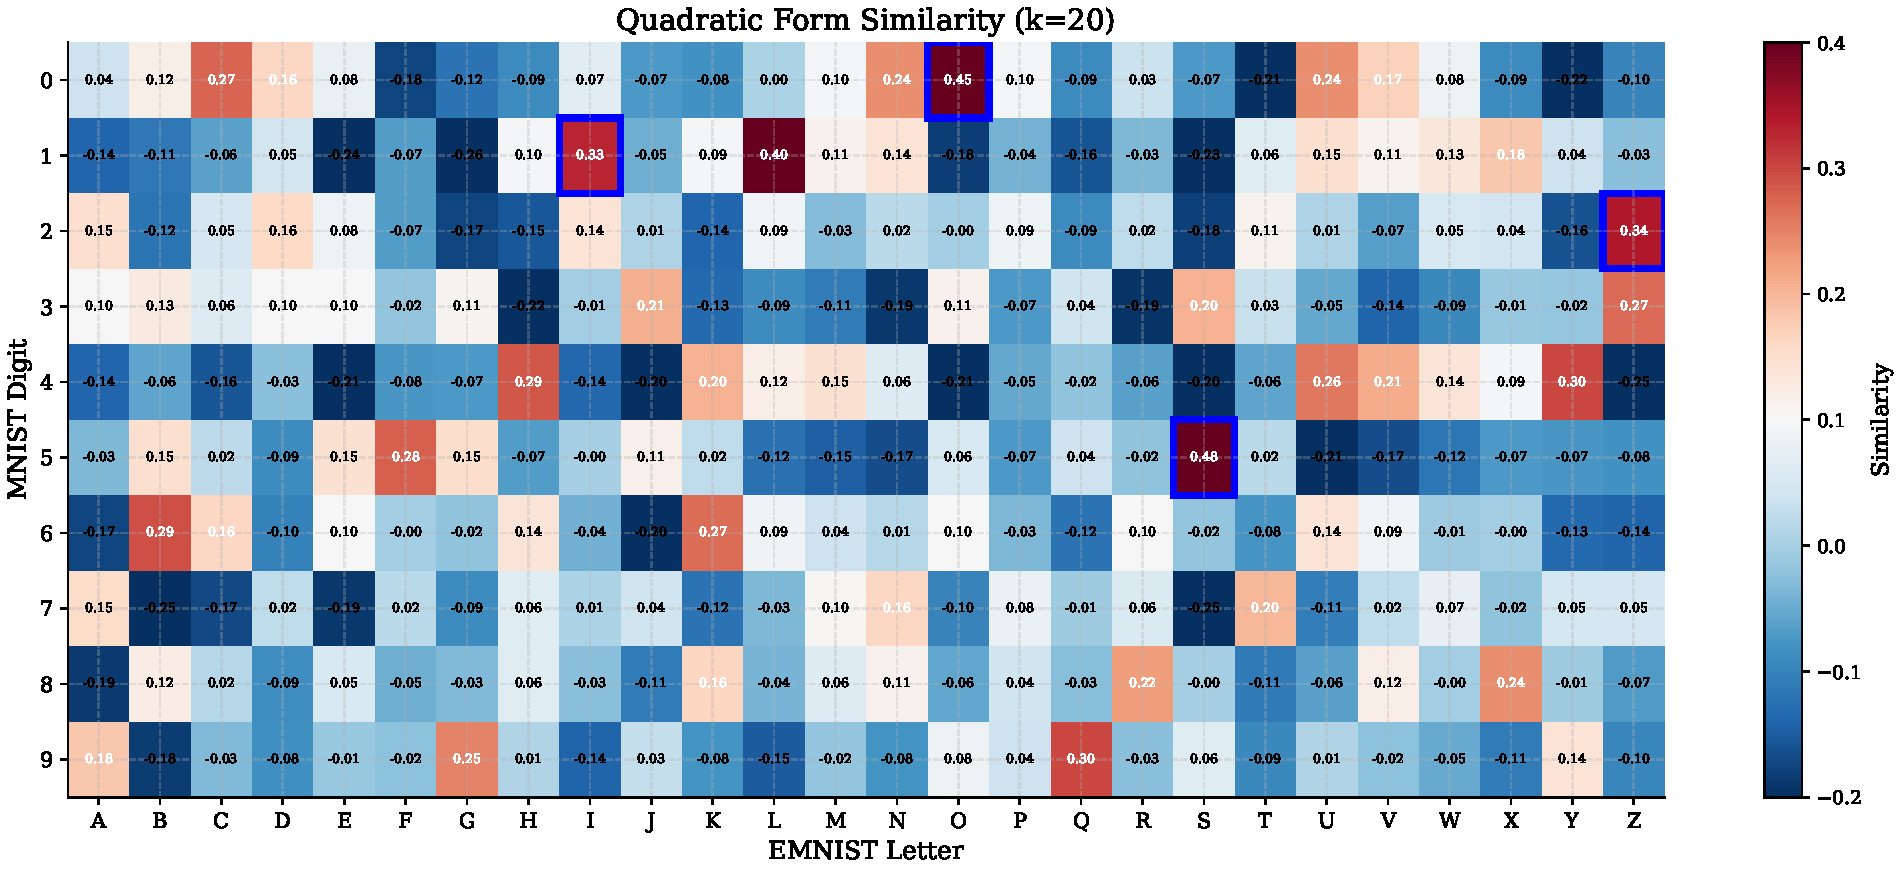
\includegraphics[width=0.85\textwidth]{../Report/figures/extension2/extension2_heatmap_quadratic_form.pdf}
            \caption{Quadratic Form Similarity Heatmap}
        \end{figure}
        \vspace{0.3cm}
        \small
        Clear discrimination: strong diagonal for MNIST vs.\ EMNIST-Digits; bright entries at shape-matched pairs (0--O, 1--I, 2--Z, 5--S)
    \end{center}
\end{frame}

\begin{frame}{Extension 1: Key Figures}
    \begin{columns}
        \column{0.5\textwidth}
        \begin{figure}
            \centering
            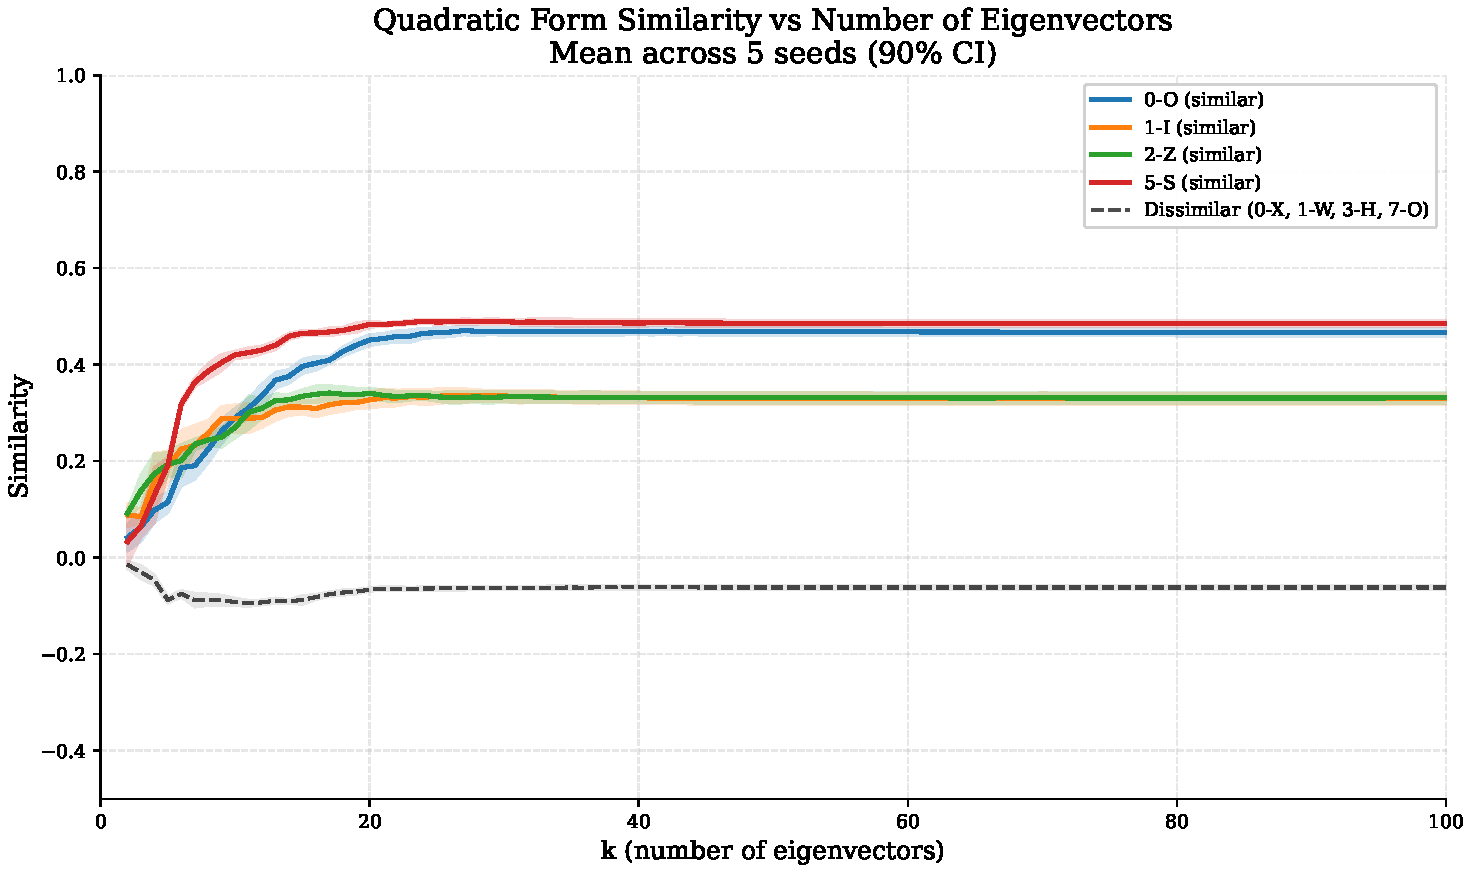
\includegraphics[width=\textwidth]{../Report/figures/extension2/extension2_similarity_vs_k_quadratic_form.pdf}
            \caption{Similarity vs Top-k Eigenvectors}
        \end{figure}
        
        \column{0.5\textwidth}
        \begin{figure}
            \centering
            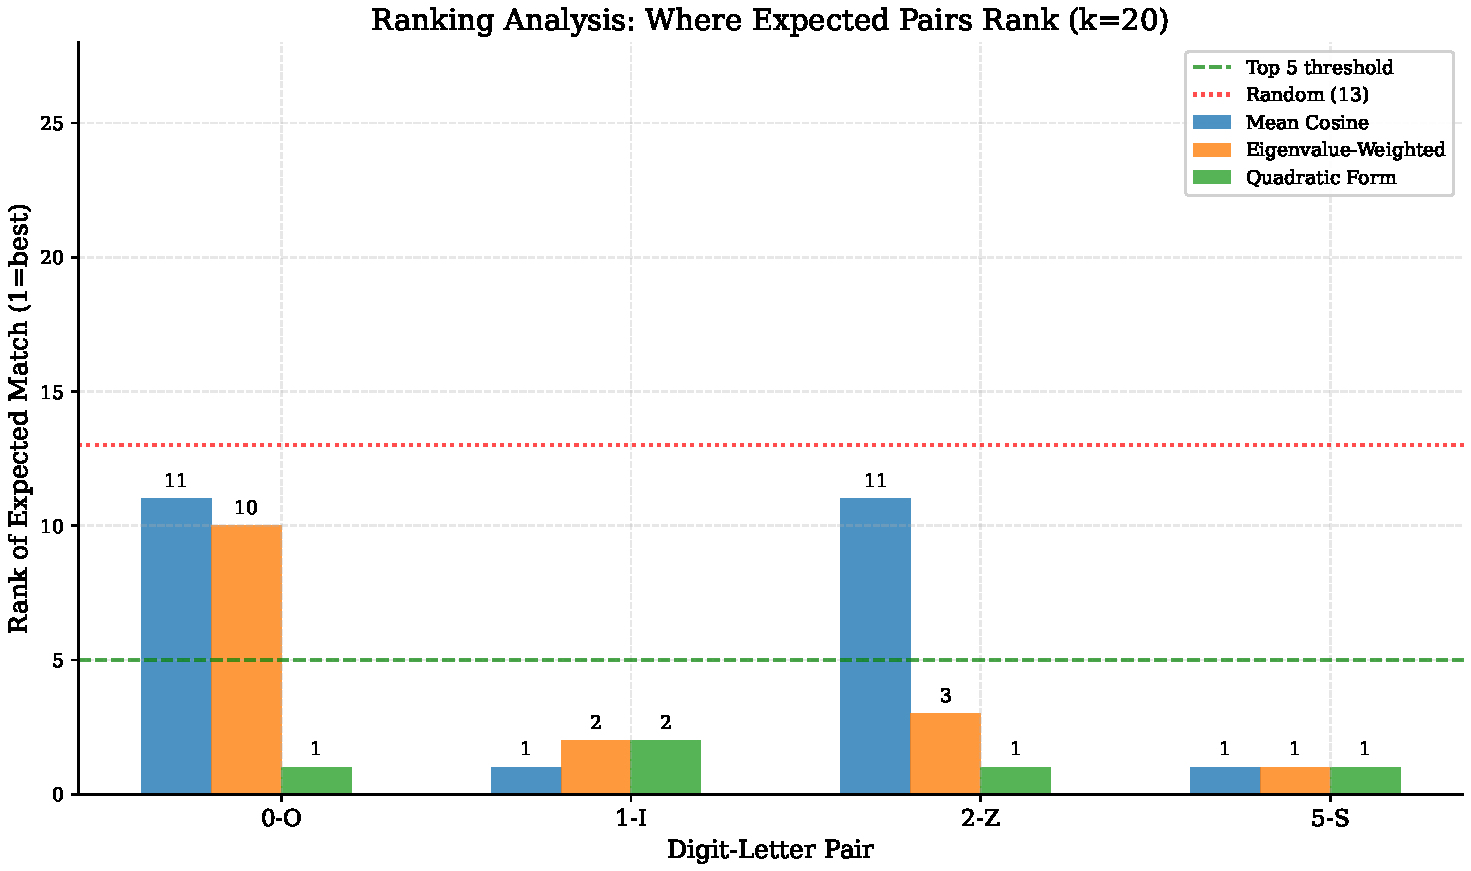
\includegraphics[width=\textwidth]{../Report/figures/extension2/extension2_ranking_analysis.pdf}
            \caption{Ranking Analysis: 3/4 similar pairs rank \#1}
        \end{figure}
    \end{columns}
\end{frame}

% Extension 2: CP-Decomposition Slides

\begin{frame}{Extension 2: CP-Decomposition}
    \begin{columns}
        \column{0.5\textwidth}
        \textbf{Motivation:}
        \begin{itemize}
            \item Post-hoc $\to$ \textbf{intrinsic} interpretability
            \item Standard eigendecomposition: orthogonality $\to$ entangled
            \item CP: disentangled features
        \end{itemize}
        
        \vspace{0.2cm}
        \textbf{CP Factorization:}
        \begin{equation*}
            W_{cij} = \sum_{r=1}^{R} \lambda_r A_{cr} B_{ir} C_{jr}
        \end{equation*}
        
        \vspace{0.2cm}
        \textbf{Key Properties:}
        \begin{itemize}
            \item No orthogonality constraint
            \item Disentangled representations
            \item Parameter reduction $\to$ faster training and scalability
        \end{itemize}
        
        \column{0.5\textwidth}
        \begin{figure}
            \centering
            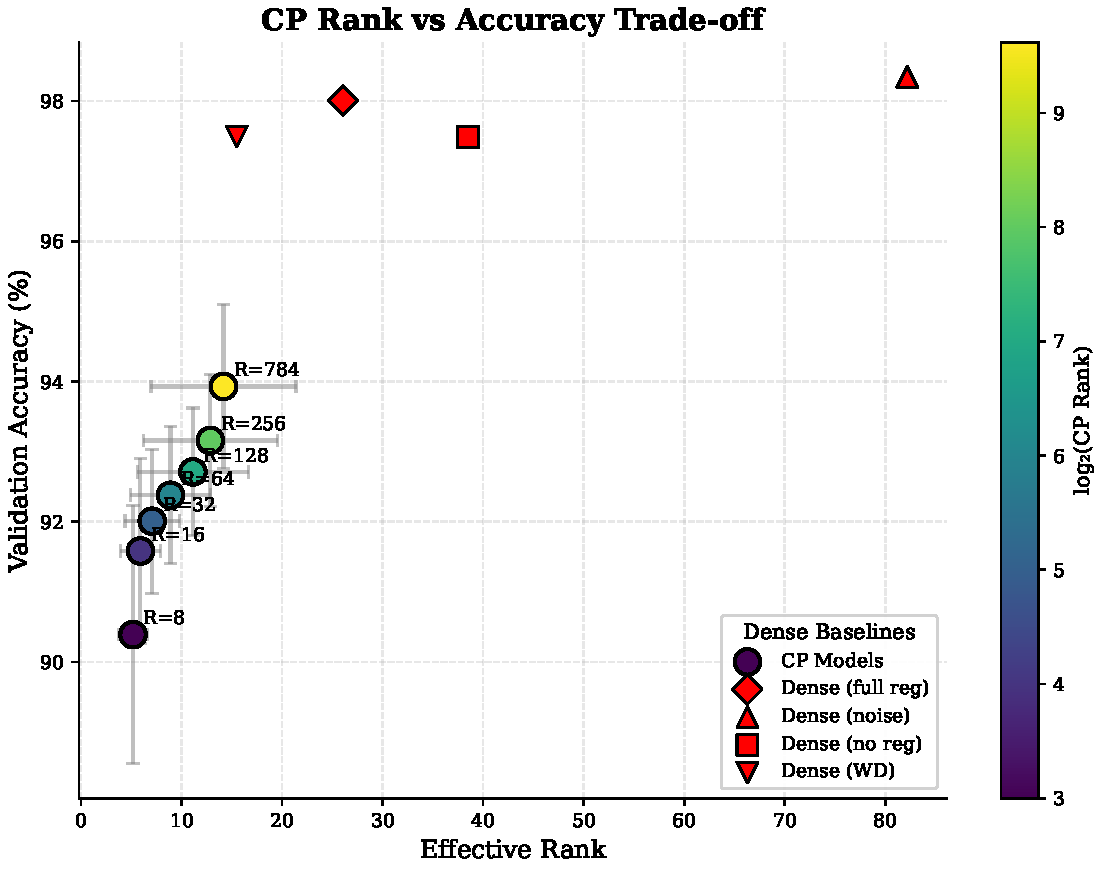
\includegraphics[width=0.95\textwidth]{../Report/figures/extension_cp/cp_rank_accuracy_tradeoff.pdf}
            \caption{Accuracy vs rank trade-off}
        \end{figure}
        
        \vspace{0.2cm}
        \textbf{Results at $R=256$:}
        \begin{itemize}
            \item Accuracy: \textbf{93.8\%}
            \item Effective rank: \textbf{17.5}
            \item vs Dense: 97.5\% (3.7 pp drop)
        \end{itemize}
    \end{columns}
\end{frame}

\begin{frame}{CP-Decomposition: Efficiency}
    \begin{center}
        \begin{table}
            \centering
            \small
            \begin{tabular}{lcccc}
                \toprule
                Experiment & Runs & Wall (h) & GPU-h & CO2 (kg) \\
                \midrule
                Vision (Section 4)$^\dagger$ & 81 & 1.22 & 1.11 & 0.039 \\
                Language (Section 5)$^\ddagger$ & 3 & 19.09 & 0.00 & 0.105 \\
                Extension 1 & 15 & 0.58 & 0.58 & 0.020 \\
                Extension 2 (CP) & 105 & 0.05 & 0.05 & 0.004 \\
                \midrule
                \textbf{Total} & \textbf{204} & \textbf{20.95} & \textbf{1.74} & \textbf{0.168} \\
                \bottomrule
            \end{tabular}
            \caption{Environmental impact (CO2 via \texttt{codecarbon})}
        \end{table}
        
        
        
    \end{center}
    
    \vspace{0.3cm}
    \textbf{Key Efficiency Gains:}
    \begin{itemize}
        \item \textbf{Parameter reduction:} $\mathcal{O}(d_{\text{hidden}} \times d_{\text{in}}^2) \to \mathcal{O}(R \times d_{\text{in}})$
        \item Average GPU-h per run: CP decomposition (0.00048) vs Vision (0.014) --- \textbf{29$\times$ more efficient}
        \item Only \textbf{3.7 pp accuracy drop} for significant parameter efficiency
    \end{itemize}
\end{frame}

\begin{frame}{CP-Decomposition: Disentangled Factors}
    \begin{figure}
        \centering
        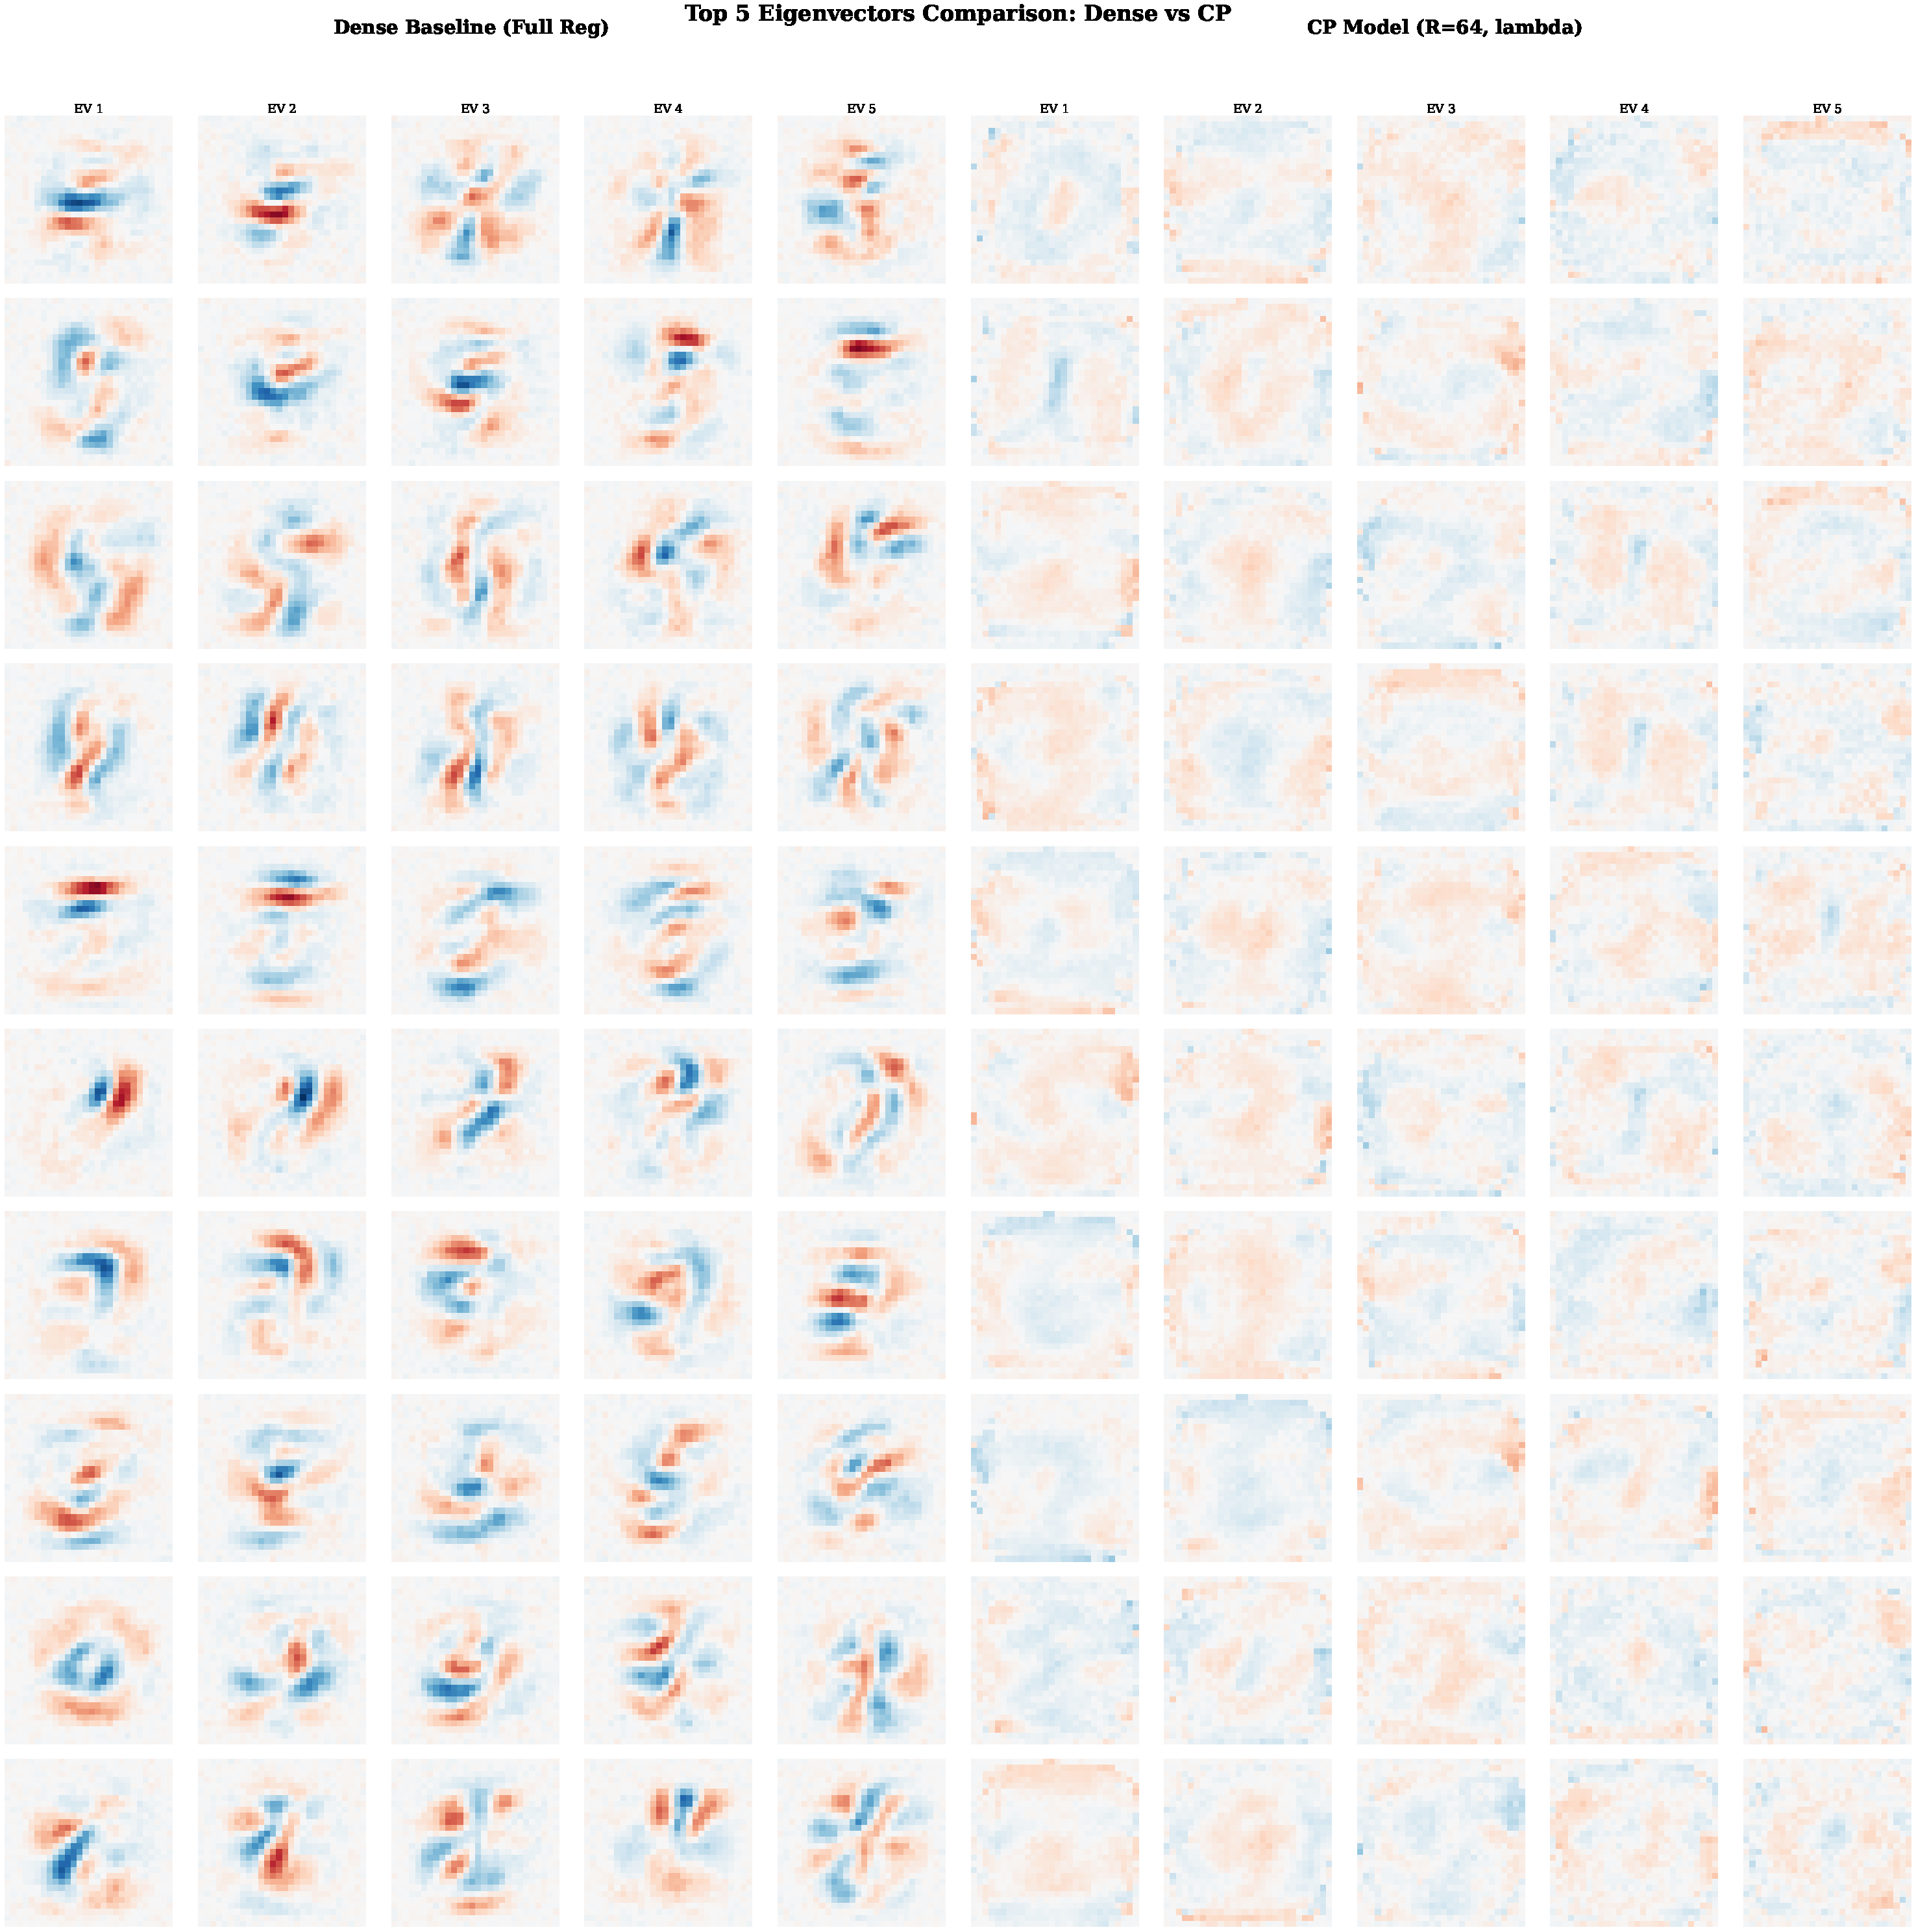
\includegraphics[width=0.65\textwidth,height=0.45\textheight,keepaspectratio]{../Report/figures/extension_cp/cp_top5_eigenvectors_comparison.pdf}
        \caption{Feature disentanglement: Dense vs.\ CP}
    \end{figure}
    
    \vspace{-0.2cm}
    \begin{columns}
        \column{0.5\textwidth}
        \small
        \textbf{Dense Eigenvectors:}
        \begin{itemize}
            \item Holistic, superimposed templates
            \item Entangled representations
        \end{itemize}
        
        \column{0.5\textwidth}
        \small
        \textbf{CP Factors:}
        \begin{itemize}
            \item Atomic, localized factors
            \item ``Parts-based'' representations
        \end{itemize}
    \end{columns}
\end{frame}

\begin{frame}
    \centering
    \vspace{2cm}
    {\Huge \textbf{Thank You!}}
    
    \vspace{1.5cm}
    {\large Questions?}
    
    \vspace{1.5cm}
    \small
    Itay Erlich, May Ben Zion, Jacob Shashoua, Sagi Schwartz
    
    \vspace{0.3cm}
    \footnotesize
    FACT-AI Course Project, University of Amsterdam
\end{frame}


% Appendix
\appendix
% Appendix Slides

\begin{frame}{Appendix: CP-Decomposition Variants}
    \begin{center}
        \Large
        \textbf{CP-Decomposition Variants}
        
        \vspace{0.5cm}
        \normalsize
        Three variants with different regularization approaches
    \end{center}
\end{frame}

\begin{frame}{Fixed CP}
    \textbf{Fixed CP:} Hard rank constraint with no additional regularization
    
    \vspace{0.5cm}
    \textbf{Characteristics:}
    \begin{itemize}
        \item Strict complexity bound: rank $R$ is fixed during training
        \item No regularization on the factors or scaling parameters
        \item Operates as a strict bottleneck
    \end{itemize}
    
    \vspace{0.5cm}
    \textbf{Results:}
    \begin{itemize}
        \item Effective rank $\sim$3.5 regardless of allocated capacity ($R \in \{32, 64, 128, 256\}$)
        \item Accuracy: $\sim$91.9\% (vs.\ 97.5\% dense)
        \item $\sim$6\% accuracy cost for extreme sparsity
    \end{itemize}
    
    \vspace{0.3cm}
    \small
    Forces extreme sparsity at the cost of accuracy
\end{frame}

\begin{frame}{Lambda CP (L1 Regularization)}
    \textbf{Lambda CP:} $L_1$ regularization on learnable scales $\lambda_r$
    
    \vspace{0.5cm}
    \textbf{Characteristics:}
    \begin{itemize}
        \item Soft sparsity via $L_1$ regularization on $\lambda_r$ parameters
        \item Allows factors to be pruned naturally during training
        \item More flexible than Fixed CP
    \end{itemize}
    
    \vspace{0.5cm}
    \textbf{Results:}
    \begin{itemize}
        \item At $R=256$: \textbf{93.8\%} accuracy
        \item Effective rank: \textbf{17.5}
        \item Comparable to dense models with weight decay (eff.\ rank 15.5)
    \end{itemize}
    
    \vspace{0.3cm}
    \small
    Provides robust middle ground: competitive accuracy with structural disentanglement
\end{frame}

\begin{frame}{Gated CP (L0 Proxy)}
    \textbf{Gated CP:} Hard sigmoid gates with $L_0$ proxy for explicit rank pruning
    
    \vspace{0.5cm}
    \textbf{Characteristics:}
    \begin{itemize}
        \item Uses $L_0$ regularization proxy: $\sum_r \sigma(\phi_r)$ approximates count of active ranks
        \item Learnable gate logits $\phi_r$ control continuous gate values (0--1)
        \item Hard sigmoid gates: $\text{clamp}(\sigma(\phi_r) \cdot 1.1 - 0.05, 0, 1)$
        \item Most flexible regularization approach
    \end{itemize}
    
    \vspace{0.5cm}
    \textbf{Results:}
    \begin{itemize}
        \item At $R=256$: \textbf{93.79\%} accuracy
        \item Effective rank: \textbf{17.35}
        \item Similar performance to Lambda CP
    \end{itemize}
    
    \vspace{0.3cm}
    \small
    Alternative approach to Lambda CP with similar performance; both provide efficient, interpretable modeling
\end{frame}


\end{document}
